\documentclass[]{book}
\usepackage{lmodern}
\usepackage{amssymb,amsmath}
\usepackage{ifxetex,ifluatex}
\usepackage{fixltx2e} % provides \textsubscript
\ifnum 0\ifxetex 1\fi\ifluatex 1\fi=0 % if pdftex
  \usepackage[T1]{fontenc}
  \usepackage[utf8]{inputenc}
\else % if luatex or xelatex
  \ifxetex
    \usepackage{mathspec}
  \else
    \usepackage{fontspec}
  \fi
  \defaultfontfeatures{Ligatures=TeX,Scale=MatchLowercase}
\fi
% use upquote if available, for straight quotes in verbatim environments
\IfFileExists{upquote.sty}{\usepackage{upquote}}{}
% use microtype if available
\IfFileExists{microtype.sty}{%
\usepackage{microtype}
\UseMicrotypeSet[protrusion]{basicmath} % disable protrusion for tt fonts
}{}
\usepackage[margin=1in]{geometry}
\usepackage{hyperref}
\hypersetup{unicode=true,
            pdftitle={A Second Semester Statistics Course with R},
            pdfauthor={Mark Greenwood and Katherine Banner},
            pdfborder={0 0 0},
            breaklinks=true}
\urlstyle{same}  % don't use monospace font for urls
\usepackage{natbib}
\bibliographystyle{apalike}
\usepackage{color}
\usepackage{fancyvrb}
\newcommand{\VerbBar}{|}
\newcommand{\VERB}{\Verb[commandchars=\\\{\}]}
\DefineVerbatimEnvironment{Highlighting}{Verbatim}{commandchars=\\\{\}}
% Add ',fontsize=\small' for more characters per line
\usepackage{framed}
\definecolor{shadecolor}{RGB}{248,248,248}
\newenvironment{Shaded}{\begin{snugshade}}{\end{snugshade}}
\newcommand{\KeywordTok}[1]{\textcolor[rgb]{0.13,0.29,0.53}{\textbf{{#1}}}}
\newcommand{\DataTypeTok}[1]{\textcolor[rgb]{0.13,0.29,0.53}{{#1}}}
\newcommand{\DecValTok}[1]{\textcolor[rgb]{0.00,0.00,0.81}{{#1}}}
\newcommand{\BaseNTok}[1]{\textcolor[rgb]{0.00,0.00,0.81}{{#1}}}
\newcommand{\FloatTok}[1]{\textcolor[rgb]{0.00,0.00,0.81}{{#1}}}
\newcommand{\ConstantTok}[1]{\textcolor[rgb]{0.00,0.00,0.00}{{#1}}}
\newcommand{\CharTok}[1]{\textcolor[rgb]{0.31,0.60,0.02}{{#1}}}
\newcommand{\SpecialCharTok}[1]{\textcolor[rgb]{0.00,0.00,0.00}{{#1}}}
\newcommand{\StringTok}[1]{\textcolor[rgb]{0.31,0.60,0.02}{{#1}}}
\newcommand{\VerbatimStringTok}[1]{\textcolor[rgb]{0.31,0.60,0.02}{{#1}}}
\newcommand{\SpecialStringTok}[1]{\textcolor[rgb]{0.31,0.60,0.02}{{#1}}}
\newcommand{\ImportTok}[1]{{#1}}
\newcommand{\CommentTok}[1]{\textcolor[rgb]{0.56,0.35,0.01}{\textit{{#1}}}}
\newcommand{\DocumentationTok}[1]{\textcolor[rgb]{0.56,0.35,0.01}{\textbf{\textit{{#1}}}}}
\newcommand{\AnnotationTok}[1]{\textcolor[rgb]{0.56,0.35,0.01}{\textbf{\textit{{#1}}}}}
\newcommand{\CommentVarTok}[1]{\textcolor[rgb]{0.56,0.35,0.01}{\textbf{\textit{{#1}}}}}
\newcommand{\OtherTok}[1]{\textcolor[rgb]{0.56,0.35,0.01}{{#1}}}
\newcommand{\FunctionTok}[1]{\textcolor[rgb]{0.00,0.00,0.00}{{#1}}}
\newcommand{\VariableTok}[1]{\textcolor[rgb]{0.00,0.00,0.00}{{#1}}}
\newcommand{\ControlFlowTok}[1]{\textcolor[rgb]{0.13,0.29,0.53}{\textbf{{#1}}}}
\newcommand{\OperatorTok}[1]{\textcolor[rgb]{0.81,0.36,0.00}{\textbf{{#1}}}}
\newcommand{\BuiltInTok}[1]{{#1}}
\newcommand{\ExtensionTok}[1]{{#1}}
\newcommand{\PreprocessorTok}[1]{\textcolor[rgb]{0.56,0.35,0.01}{\textit{{#1}}}}
\newcommand{\AttributeTok}[1]{\textcolor[rgb]{0.77,0.63,0.00}{{#1}}}
\newcommand{\RegionMarkerTok}[1]{{#1}}
\newcommand{\InformationTok}[1]{\textcolor[rgb]{0.56,0.35,0.01}{\textbf{\textit{{#1}}}}}
\newcommand{\WarningTok}[1]{\textcolor[rgb]{0.56,0.35,0.01}{\textbf{\textit{{#1}}}}}
\newcommand{\AlertTok}[1]{\textcolor[rgb]{0.94,0.16,0.16}{{#1}}}
\newcommand{\ErrorTok}[1]{\textcolor[rgb]{0.64,0.00,0.00}{\textbf{{#1}}}}
\newcommand{\NormalTok}[1]{{#1}}
\usepackage{longtable,booktabs}
\usepackage{graphicx,grffile}
\makeatletter
\def\maxwidth{\ifdim\Gin@nat@width>\linewidth\linewidth\else\Gin@nat@width\fi}
\def\maxheight{\ifdim\Gin@nat@height>\textheight\textheight\else\Gin@nat@height\fi}
\makeatother
% Scale images if necessary, so that they will not overflow the page
% margins by default, and it is still possible to overwrite the defaults
% using explicit options in \includegraphics[width, height, ...]{}
\setkeys{Gin}{width=\maxwidth,height=\maxheight,keepaspectratio}
\IfFileExists{parskip.sty}{%
\usepackage{parskip}
}{% else
\setlength{\parindent}{0pt}
\setlength{\parskip}{6pt plus 2pt minus 1pt}
}
\setlength{\emergencystretch}{3em}  % prevent overfull lines
\providecommand{\tightlist}{%
  \setlength{\itemsep}{0pt}\setlength{\parskip}{0pt}}
\setcounter{secnumdepth}{5}
% Redefines (sub)paragraphs to behave more like sections
\ifx\paragraph\undefined\else
\let\oldparagraph\paragraph
\renewcommand{\paragraph}[1]{\oldparagraph{#1}\mbox{}}
\fi
\ifx\subparagraph\undefined\else
\let\oldsubparagraph\subparagraph
\renewcommand{\subparagraph}[1]{\oldsubparagraph{#1}\mbox{}}
\fi

%%% Use protect on footnotes to avoid problems with footnotes in titles
\let\rmarkdownfootnote\footnote%
\def\footnote{\protect\rmarkdownfootnote}

%%% Change title format to be more compact
\usepackage{titling}

% Create subtitle command for use in maketitle
\newcommand{\subtitle}[1]{
  \posttitle{
    \begin{center}\large#1\end{center}
    }
}

\setlength{\droptitle}{-2em}
  \title{A Second Semester Statistics Course with R}
  \pretitle{\vspace{\droptitle}\centering\huge}
  \posttitle{\par}
  \author{Mark Greenwood and Katherine Banner}
  \preauthor{\centering\large\emph}
  \postauthor{\par}
  \predate{\centering\large\emph}
  \postdate{\par}
  \date{2017-05-26}

\usepackage{booktabs}

\begin{document}
\maketitle

{
\setcounter{tocdepth}{1}
\tableofcontents
}
\chapter*{Acknowledgments}\label{acknowledgments}
\addcontentsline{toc}{chapter}{Acknowledgments}

\chapter{Placeholder}\label{placeholder}

\chapter{(R)e-Introduction to
statistics}\label{re-introduction-to-statistics}

The previous material served to get us started in R and to get a quick
review of same basic descriptive statistics. Now we will begin to engage
some new material and exploit the power of R to do some statistical
inference. Because inference is one of the hardest topics to master in
statistics, we will also review some basic terminology that is required
to move forward in learning more sophisticated statistical methods. To
keep this ``review'' as short as possible, we will not consider every
situation you learned in introductory statistics and instead focus
exclusively on the situation where we have a quantitative response
variable measured on two groups, adding a new graphic called a ``bean
plot'' to help us see the differences in the observations in the groups.

\section{Histograms, boxplots, and density curves}\label{section_2-1}

Part of learning statistics is learning to correctly use the
terminology, some of which is used colloquially differently than it is
used in formal statistical settings. The most commonly ``misused'' term
is \textbf{\emph{data}}. In statistical parlance, we want to note the
plurality of data. Specifically, \textbf{\emph{datum}} is a single
measurement, possibly on multiple random variables, and so it is
appropriate to say that ``\textbf{a datum is\ldots{}}''. Once we move to
discussing data, we are now referring to more than one observation,
again on one, or possibly more than one, random variable, and so we need
to use ``\textbf{data are\ldots{}}'' when talking about our
observations. We want to distinguish our use of the term ``data'' from
its more colloquial\footnote{You will more typically hear ``data is''
  but that more often refers to information, sometimes even statistical
  summaries of data sets, than to observations collected as part of a
  study, suggesting the confusion of this term in the general public. We
  will explore a data set in Chapter 4 related to perceptions of this
  issue collected by researchers at \url{http://fivethirtyeight.com/}.}
usage that often involves treating it as singular. In a statistical
setting ``data'' refers to measurements of our cases or units. When we
summarize the results of a study (say providing the mean and SD), that
information is not ``data''. We used our data to generate that
information. Sometimes we also use the term ``data set'' to refer to all
our observations and this is a singular term to refer to the group of
observations and this makes it really easy to make mistakes on the usage
of this term.

It is also really important to note that \textbf{\emph{variables}} have
to vary -- if you measure the sex of your subjects but are only
measuring females, then you do not have a ``variable''. You may not know
if you have real variability in a ``variable'' until you explore the
results you obtained.

The last, but probably most important, aspect of data is the context of
the measurement. The ``who, what, when, and where'' of the collection of
the observations is critical to the sort of conclusions we can make
based on the results. The information on the study design provides
information required to assess the scope of inference of the study.
Generally, remember to think about the research questions the
researchers were trying to answer and whether their study actually would
answer those questions. There are no formulas to help us sort some of
these things out, just critical thinking about the context of the
measurements.

To make this concrete, consider the data collected from a study
(Plaster, 1989) to investigate whether perceived physical attractiveness
had an impact on the sentences or perceived seriousness of a crime that
male jurors might give to female defendants. The researchers showed the
participants in the study (men who volunteered from a prison) pictures
of one of three young women. Each picture had previously been decided to
be either beautiful, average, or unattractive by the researchers. Each
``juror'' was randomly assigned to one of three levels of this factor
(which is a categorical predictor or explanatory variable) and then each
rated their picture on a variety of traits such as how warm or sincere
the woman appeared. Finally, they were told the women had committed a
crime (also randomly assigned to either be told she committed a burglary
or a swindle) and were asked to rate the seriousness of the crime and
provide a suggested length of sentence. We will bypass some aspects of
their research and just focus on differences in the sentence suggested
among the three pictures. To get a sense of these data, let's consider
the first and last parts of the data set:

\begin{longtable}[]{@{}lllllll@{}}
\toprule
\begin{minipage}[b]{0.11\columnwidth}\raggedright\strut
Subject\strut
\end{minipage} & \begin{minipage}[b]{0.13\columnwidth}\raggedright\strut
Attr\strut
\end{minipage} & \begin{minipage}[b]{0.13\columnwidth}\raggedright\strut
Crime\strut
\end{minipage} & \begin{minipage}[b]{0.09\columnwidth}\raggedright\strut
Years\strut
\end{minipage} & \begin{minipage}[b]{0.11\columnwidth}\raggedright\strut
Serious\strut
\end{minipage} & \begin{minipage}[b]{0.15\columnwidth}\raggedright\strut
independent\strut
\end{minipage} & \begin{minipage}[b]{0.09\columnwidth}\raggedright\strut
Sincere\strut
\end{minipage}\tabularnewline
\midrule
\endhead
\begin{minipage}[t]{0.11\columnwidth}\raggedright\strut
1\strut
\end{minipage} & \begin{minipage}[t]{0.13\columnwidth}\raggedright\strut
Beautiful\strut
\end{minipage} & \begin{minipage}[t]{0.13\columnwidth}\raggedright\strut
Burglary\strut
\end{minipage} & \begin{minipage}[t]{0.09\columnwidth}\raggedright\strut
10\strut
\end{minipage} & \begin{minipage}[t]{0.11\columnwidth}\raggedright\strut
8\strut
\end{minipage} & \begin{minipage}[t]{0.15\columnwidth}\raggedright\strut
9\strut
\end{minipage} & \begin{minipage}[t]{0.09\columnwidth}\raggedright\strut
8\strut
\end{minipage}\tabularnewline
\begin{minipage}[t]{0.11\columnwidth}\raggedright\strut
2\strut
\end{minipage} & \begin{minipage}[t]{0.13\columnwidth}\raggedright\strut
Beautiful\strut
\end{minipage} & \begin{minipage}[t]{0.13\columnwidth}\raggedright\strut
Burglary\strut
\end{minipage} & \begin{minipage}[t]{0.09\columnwidth}\raggedright\strut
3\strut
\end{minipage} & \begin{minipage}[t]{0.11\columnwidth}\raggedright\strut
8\strut
\end{minipage} & \begin{minipage}[t]{0.15\columnwidth}\raggedright\strut
9\strut
\end{minipage} & \begin{minipage}[t]{0.09\columnwidth}\raggedright\strut
3\strut
\end{minipage}\tabularnewline
\begin{minipage}[t]{0.11\columnwidth}\raggedright\strut
3\strut
\end{minipage} & \begin{minipage}[t]{0.13\columnwidth}\raggedright\strut
Beautiful\strut
\end{minipage} & \begin{minipage}[t]{0.13\columnwidth}\raggedright\strut
Burglary\strut
\end{minipage} & \begin{minipage}[t]{0.09\columnwidth}\raggedright\strut
5\strut
\end{minipage} & \begin{minipage}[t]{0.11\columnwidth}\raggedright\strut
5\strut
\end{minipage} & \begin{minipage}[t]{0.15\columnwidth}\raggedright\strut
6\strut
\end{minipage} & \begin{minipage}[t]{0.09\columnwidth}\raggedright\strut
3\strut
\end{minipage}\tabularnewline
\begin{minipage}[t]{0.11\columnwidth}\raggedright\strut
4\strut
\end{minipage} & \begin{minipage}[t]{0.13\columnwidth}\raggedright\strut
Beautiful\strut
\end{minipage} & \begin{minipage}[t]{0.13\columnwidth}\raggedright\strut
Burglary\strut
\end{minipage} & \begin{minipage}[t]{0.09\columnwidth}\raggedright\strut
1\strut
\end{minipage} & \begin{minipage}[t]{0.11\columnwidth}\raggedright\strut
3\strut
\end{minipage} & \begin{minipage}[t]{0.15\columnwidth}\raggedright\strut
9\strut
\end{minipage} & \begin{minipage}[t]{0.09\columnwidth}\raggedright\strut
8\strut
\end{minipage}\tabularnewline
\begin{minipage}[t]{0.11\columnwidth}\raggedright\strut
5\strut
\end{minipage} & \begin{minipage}[t]{0.13\columnwidth}\raggedright\strut
Beautiful\strut
\end{minipage} & \begin{minipage}[t]{0.13\columnwidth}\raggedright\strut
Burglary\strut
\end{minipage} & \begin{minipage}[t]{0.09\columnwidth}\raggedright\strut
7\strut
\end{minipage} & \begin{minipage}[t]{0.11\columnwidth}\raggedright\strut
9\strut
\end{minipage} & \begin{minipage}[t]{0.15\columnwidth}\raggedright\strut
5\strut
\end{minipage} & \begin{minipage}[t]{0.09\columnwidth}\raggedright\strut
1\strut
\end{minipage}\tabularnewline
\begin{minipage}[t]{0.11\columnwidth}\raggedright\strut
\ldots{}\strut
\end{minipage} & \begin{minipage}[t]{0.13\columnwidth}\raggedright\strut
\ldots{}\strut
\end{minipage} & \begin{minipage}[t]{0.13\columnwidth}\raggedright\strut
\ldots{}\strut
\end{minipage} & \begin{minipage}[t]{0.09\columnwidth}\raggedright\strut
\ldots{}\strut
\end{minipage} & \begin{minipage}[t]{0.11\columnwidth}\raggedright\strut
\ldots{}\strut
\end{minipage} & \begin{minipage}[t]{0.15\columnwidth}\raggedright\strut
\ldots{}\strut
\end{minipage} & \begin{minipage}[t]{0.09\columnwidth}\raggedright\strut
\ldots{}\strut
\end{minipage}\tabularnewline
\begin{minipage}[t]{0.11\columnwidth}\raggedright\strut
108\strut
\end{minipage} & \begin{minipage}[t]{0.13\columnwidth}\raggedright\strut
Average\strut
\end{minipage} & \begin{minipage}[t]{0.13\columnwidth}\raggedright\strut
Swindle\strut
\end{minipage} & \begin{minipage}[t]{0.09\columnwidth}\raggedright\strut
3\strut
\end{minipage} & \begin{minipage}[t]{0.11\columnwidth}\raggedright\strut
3\strut
\end{minipage} & \begin{minipage}[t]{0.15\columnwidth}\raggedright\strut
5\strut
\end{minipage} & \begin{minipage}[t]{0.09\columnwidth}\raggedright\strut
4\strut
\end{minipage}\tabularnewline
\begin{minipage}[t]{0.11\columnwidth}\raggedright\strut
109\strut
\end{minipage} & \begin{minipage}[t]{0.13\columnwidth}\raggedright\strut
Average\strut
\end{minipage} & \begin{minipage}[t]{0.13\columnwidth}\raggedright\strut
Swindle\strut
\end{minipage} & \begin{minipage}[t]{0.09\columnwidth}\raggedright\strut
3\strut
\end{minipage} & \begin{minipage}[t]{0.11\columnwidth}\raggedright\strut
2\strut
\end{minipage} & \begin{minipage}[t]{0.15\columnwidth}\raggedright\strut
9\strut
\end{minipage} & \begin{minipage}[t]{0.09\columnwidth}\raggedright\strut
9\strut
\end{minipage}\tabularnewline
\begin{minipage}[t]{0.11\columnwidth}\raggedright\strut
110\strut
\end{minipage} & \begin{minipage}[t]{0.13\columnwidth}\raggedright\strut
Average\strut
\end{minipage} & \begin{minipage}[t]{0.13\columnwidth}\raggedright\strut
Swindle\strut
\end{minipage} & \begin{minipage}[t]{0.09\columnwidth}\raggedright\strut
2\strut
\end{minipage} & \begin{minipage}[t]{0.11\columnwidth}\raggedright\strut
1\strut
\end{minipage} & \begin{minipage}[t]{0.15\columnwidth}\raggedright\strut
8\strut
\end{minipage} & \begin{minipage}[t]{0.09\columnwidth}\raggedright\strut
8\strut
\end{minipage}\tabularnewline
\begin{minipage}[t]{0.11\columnwidth}\raggedright\strut
111\strut
\end{minipage} & \begin{minipage}[t]{0.13\columnwidth}\raggedright\strut
Average\strut
\end{minipage} & \begin{minipage}[t]{0.13\columnwidth}\raggedright\strut
Swindle\strut
\end{minipage} & \begin{minipage}[t]{0.09\columnwidth}\raggedright\strut
7\strut
\end{minipage} & \begin{minipage}[t]{0.11\columnwidth}\raggedright\strut
4\strut
\end{minipage} & \begin{minipage}[t]{0.15\columnwidth}\raggedright\strut
9\strut
\end{minipage} & \begin{minipage}[t]{0.09\columnwidth}\raggedright\strut
1\strut
\end{minipage}\tabularnewline
\begin{minipage}[t]{0.11\columnwidth}\raggedright\strut
112\strut
\end{minipage} & \begin{minipage}[t]{0.13\columnwidth}\raggedright\strut
Average\strut
\end{minipage} & \begin{minipage}[t]{0.13\columnwidth}\raggedright\strut
Swindle\strut
\end{minipage} & \begin{minipage}[t]{0.09\columnwidth}\raggedright\strut
6\strut
\end{minipage} & \begin{minipage}[t]{0.11\columnwidth}\raggedright\strut
3\strut
\end{minipage} & \begin{minipage}[t]{0.15\columnwidth}\raggedright\strut
5\strut
\end{minipage} & \begin{minipage}[t]{0.09\columnwidth}\raggedright\strut
2\strut
\end{minipage}\tabularnewline
\begin{minipage}[t]{0.11\columnwidth}\raggedright\strut
113\strut
\end{minipage} & \begin{minipage}[t]{0.13\columnwidth}\raggedright\strut
Average\strut
\end{minipage} & \begin{minipage}[t]{0.13\columnwidth}\raggedright\strut
Swindle\strut
\end{minipage} & \begin{minipage}[t]{0.09\columnwidth}\raggedright\strut
12\strut
\end{minipage} & \begin{minipage}[t]{0.11\columnwidth}\raggedright\strut
9\strut
\end{minipage} & \begin{minipage}[t]{0.15\columnwidth}\raggedright\strut
9\strut
\end{minipage} & \begin{minipage}[t]{0.09\columnwidth}\raggedright\strut
1\strut
\end{minipage}\tabularnewline
\begin{minipage}[t]{0.11\columnwidth}\raggedright\strut
114\strut
\end{minipage} & \begin{minipage}[t]{0.13\columnwidth}\raggedright\strut
Average\strut
\end{minipage} & \begin{minipage}[t]{0.13\columnwidth}\raggedright\strut
Swindle\strut
\end{minipage} & \begin{minipage}[t]{0.09\columnwidth}\raggedright\strut
8\strut
\end{minipage} & \begin{minipage}[t]{0.11\columnwidth}\raggedright\strut
8\strut
\end{minipage} & \begin{minipage}[t]{0.15\columnwidth}\raggedright\strut
1\strut
\end{minipage} & \begin{minipage}[t]{0.09\columnwidth}\raggedright\strut
5\strut
\end{minipage}\tabularnewline
\bottomrule
\end{longtable}

When working with data, we should always start with summarizing the
sample size. We will use \textbf{\emph{n}} for the number of subjects in
the sample and denote the population size (if available) with
\textbf{\emph{N}}. Here, the sample size is \textbf{\emph{n=114}}. In
this situation, we do not have a random sample from a population (these
were volunteers from the population of prisoners at the particular
prison) so we cannot make inferences to a larger group. But we can
assess whether there is a \textbf{\emph{causal effect}}\footnote{As
  noted previously, we reserve the term ``effect'' for situations where
  random assignment allows us to consider causality as the reason for
  the differences in the response variable among levels of the
  explanatory variable, but this is only the case if we find evidence
  against the null hypothesis of no difference in the groups.}: if
sufficient evidence is found to conclude that there is some difference
in the responses across the treated groups, we can attribute those
differences to the treatments applied, since the groups should be same
otherwise due to the pictures being randomly assigned to the ``jurors''.
The story of the data set ? that it was collected on prisoners --
becomes pretty important in thinking about the ramifications of any
results. Are male prisoners different from the population of college
males or all residents of a state such as Montana? If so, then we should
not assume that the detected differences, if detected, would also exist
in some other group of male subjects. The lack of a random sample makes
it impossible to assume that this set of prisoners might be like other
prisoners. So there are definite limitations to the inferences in the
following results. But it is still interesting to see if the pictures
caused a difference in the suggested mean sentences, even though the
inferences are limited to this group of prisoners. If this had been an
observational study (suppose that the prisoners could select one of the
three pictures), then we would have to avoid any of the ``causal''
language that we can consider here because the pictures were not
randomly assigned to the subjects. Without random assignment, the
explanatory variable of picture choice could be
\textbf{\emph{confounded}} with another characteristic of prisoners that
was related to which picture they selected and the rating they provided.
Confounding is not the only reason to avoid causal statements with
non-random assignment but the inability to separate the effect of other
variables (measured or unmeasured) from the differences we are observing
means that our inferences in these situations need to be carefully
stated.

Instead of loading this data set into R using the ``Import Dataset''
functionality, we can load an R package that contains the data, making
for easy access to this data set. The package called \texttt{heplots}
contains a data set called MockJury that contains the results of the
study. We also rely the R package called \texttt{mosaic} (Pruim, Kaplan,
and Horton, 2016) that was introduced previously. First (but only once),
you need to install both packages, which can be done either using the
Packages tab in the lower right panel of R-studio or using the
\texttt{install.packages} function with quotes around the package name:

\begin{verbatim}
> install. packages("heplots")
\end{verbatim}

After making sure that both packages are installed, we use the
\texttt{require} function around the package name (no quotes now!) to
load the package, something that you need to do any time you want to use
features of a package.

\begin{Shaded}
\begin{Highlighting}[]
\KeywordTok{require}\NormalTok{(heplots)}
\KeywordTok{require}\NormalTok{(mosaic)}
\end{Highlighting}
\end{Shaded}

There will be some results of the loading process that may discuss
loading other required packages. If the output says that it needs a
package that is unavailable, then follow the same process noted above to
install that package as well.

To load the data set that is available in an active package, we use the
\texttt{data} function.

\begin{Shaded}
\begin{Highlighting}[]
\KeywordTok{data}\NormalTok{(MockJury)}
\end{Highlighting}
\end{Shaded}

Now there will be a data.frame called \texttt{MockJury} available for us
to analyze and some information about it in the Environment tab. Again,
we can find out more about the data set in a couple of ways. First, we
can use the \texttt{View} function to provide a spreadsheet type of
display in the upper left panel. Second, we can use the \texttt{head}
and \texttt{tail} functions to print out the beginning and end of the
data set. Because there are so many variables, it may wrap around to
show all the columns.

\begin{Shaded}
\begin{Highlighting}[]
\KeywordTok{View}\NormalTok{(MockJury)}
\KeywordTok{head}\NormalTok{(MockJury)}
\end{Highlighting}
\end{Shaded}

\begin{verbatim}
##        Attr    Crime Years Serious exciting calm independent sincere warm
## 1 Beautiful Burglary    10       8        6    9           9       8    5
## 2 Beautiful Burglary     3       8        9    5           9       3    5
## 3 Beautiful Burglary     5       5        3    4           6       3    6
## 4 Beautiful Burglary     1       3        3    6           9       8    8
## 5 Beautiful Burglary     7       9        1    1           5       1    8
## 6 Beautiful Burglary     7       9        1    5           7       5    8
##   phyattr sociable kind intelligent strong sophisticated happy ownPA
## 1       9        9    9           6      9             9     5     9
## 2       9        9    4           9      5             5     5     7
## 3       7        4    2           4      5             4     5     5
## 4       9        9    9           9      9             9     9     9
## 5       8        9    4           7      9             9     8     7
## 6       8        9    5           8      9             9     9     9
\end{verbatim}

\begin{Shaded}
\begin{Highlighting}[]
\KeywordTok{tail}\NormalTok{(MockJury)}
\end{Highlighting}
\end{Shaded}

\begin{verbatim}
##        Attr   Crime Years Serious exciting calm independent sincere warm
## 109 Average Swindle     3       2        7    6           9       9    6
## 110 Average Swindle     2       1        8    8           8       8    8
## 111 Average Swindle     7       4        1    6           9       1    1
## 112 Average Swindle     6       3        5    3           5       2    4
## 113 Average Swindle    12       9        1    9           9       1    1
## 114 Average Swindle     8       8        1    9           1       5    1
##     phyattr sociable kind intelligent strong sophisticated happy ownPA
## 109       4        7    6           8      6             5     7     2
## 110       8        9    9           9      9             9     9     6
## 111       1        9    4           1      1             1     1     9
## 112       1        4    9           3      3             9     5     3
## 113       1        9    1           9      9             1     9     1
## 114       1        9    1           1      9             5     1     1
\end{verbatim}

When data sets are loaded from packages, there is often extra
documentation available about the data set which can be accessed using
the help function. In this case, it will bring up a screen with
information about the study and each variable that was measured.

\begin{Shaded}
\begin{Highlighting}[]
\KeywordTok{help}\NormalTok{(MockJury)}
\end{Highlighting}
\end{Shaded}

The help function is also useful with functions in R to help you
understand options and, at the bottom of the help, see examples of using
the function.

With many variables in a data set, it is often useful to get some quick
information about all of them; the \texttt{summary} function provides
useful information whether the variables are categorical or quantitative
and notes if any values were missing.

\begin{Shaded}
\begin{Highlighting}[]
\KeywordTok{summary}\NormalTok{(MockJury)}
\end{Highlighting}
\end{Shaded}

\begin{verbatim}
##            Attr         Crime        Years           Serious     
##  Beautiful   :39   Burglary:59   Min.   : 1.000   Min.   :1.000  
##  Average     :38   Swindle :55   1st Qu.: 2.000   1st Qu.:3.000  
##  Unattractive:37                 Median : 3.000   Median :5.000  
##                                  Mean   : 4.693   Mean   :5.018  
##                                  3rd Qu.: 7.000   3rd Qu.:6.750  
##                                  Max.   :15.000   Max.   :9.000  
##     exciting          calm        independent       sincere     
##  Min.   :1.000   Min.   :1.000   Min.   :1.000   Min.   :1.000  
##  1st Qu.:3.000   1st Qu.:4.250   1st Qu.:5.000   1st Qu.:3.000  
##  Median :5.000   Median :6.500   Median :6.500   Median :5.000  
##  Mean   :4.658   Mean   :5.982   Mean   :6.132   Mean   :4.789  
##  3rd Qu.:6.000   3rd Qu.:8.000   3rd Qu.:8.000   3rd Qu.:7.000  
##  Max.   :9.000   Max.   :9.000   Max.   :9.000   Max.   :9.000  
##       warm         phyattr        sociable          kind      
##  Min.   :1.00   Min.   :1.00   Min.   :1.000   Min.   :1.000  
##  1st Qu.:2.00   1st Qu.:2.00   1st Qu.:5.000   1st Qu.:3.000  
##  Median :5.00   Median :5.00   Median :7.000   Median :5.000  
##  Mean   :4.57   Mean   :4.93   Mean   :6.132   Mean   :4.728  
##  3rd Qu.:7.00   3rd Qu.:8.00   3rd Qu.:8.000   3rd Qu.:7.000  
##  Max.   :9.00   Max.   :9.00   Max.   :9.000   Max.   :9.000  
##   intelligent        strong      sophisticated       happy      
##  Min.   :1.000   Min.   :1.000   Min.   :1.000   Min.   :1.000  
##  1st Qu.:4.000   1st Qu.:4.000   1st Qu.:3.250   1st Qu.:3.000  
##  Median :7.000   Median :6.000   Median :5.000   Median :5.000  
##  Mean   :6.096   Mean   :5.649   Mean   :5.061   Mean   :5.061  
##  3rd Qu.:8.750   3rd Qu.:7.000   3rd Qu.:7.000   3rd Qu.:7.000  
##  Max.   :9.000   Max.   :9.000   Max.   :9.000   Max.   :9.000  
##      ownPA      
##  Min.   :1.000  
##  1st Qu.:5.000  
##  Median :6.000  
##  Mean   :6.377  
##  3rd Qu.:9.000  
##  Max.   :9.000
\end{verbatim}

If we take a few moments to explore the output we can discover some
useful aspects of the data set. The output is organized by variable,
providing summary information based on the type of variable, either
counts by category for categorical variables \texttt{Attr}\\
and \texttt{Crime} mean for quantitative variables. If present, you
would also get a count ofmissing values that are called ``NAs'' in R.
For the first variable, called \texttt{Attr} in the data.frame and that
we might we find counts of the number of subjects shown each picture:
37/114 viewed the ``Unattractive'' picture, 38 viewed ``Average'', and
39 viewed ``Beautiful''. We can also see that suggested prison sentences
(data.frame variable \texttt{Years} ) ranged from 1 year to 15 years
with a median of 3 years. It seems that all the other variables except
for \emph{Crime} (type of crime that they were told the pictured woman
committed) contained responses between 1 and 9 based on rating scales
from 1 = low to 9 = high.

To accompany the numerical summaries, histograms, and boxplots can
provide some initial information on the shape of the distribution of the
responses for the Figure \ref{fig:Figure2-1} contains the histogram and
boxplot of Years, ignoring any information on which picture the
``jurors'' were shown. The calls to the two plotting functions are
enhanced slightly to add better labels.



\begin{Shaded}
\begin{Highlighting}[]
\KeywordTok{hist}\NormalTok{(MockJury$Years, }\DataTypeTok{xlab=}\StringTok{"Years"}\NormalTok{, }\DataTypeTok{labels=}\NormalTok{T, }\DataTypeTok{main=}\StringTok{"Histogram of Years"}\NormalTok{)}
\KeywordTok{boxplot}\NormalTok{(MockJury$Years, }\DataTypeTok{ylab=}\StringTok{"Years"}\NormalTok{, }\DataTypeTok{main=}\StringTok{"Boxplot of Years"}\NormalTok{)}
\end{Highlighting}
\end{Shaded}

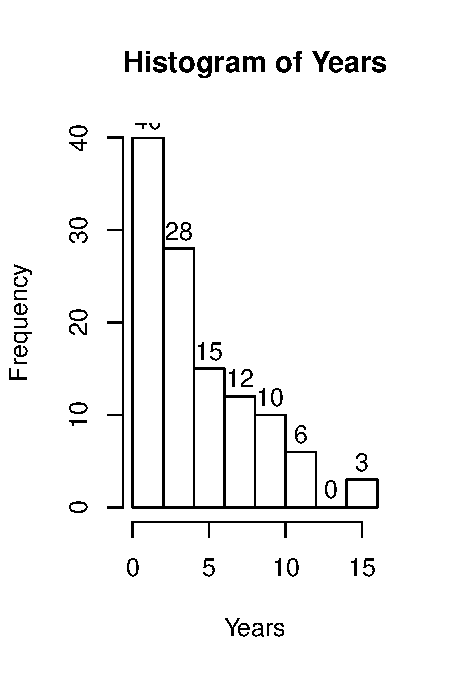
\includegraphics{GreenwoodBanner_files/figure-latex/Figure2-1-1.pdf}
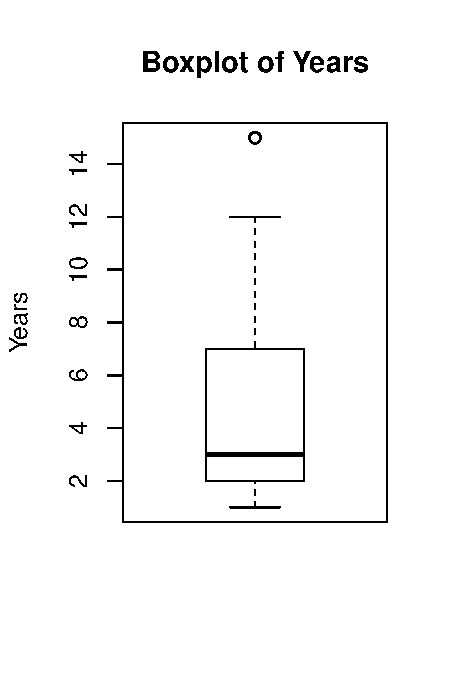
\includegraphics{GreenwoodBanner_files/figure-latex/Figure2-1-2.pdf}

The distribution appears to have a strong right skew with three
observations at 15 years flagged as potential outliers. You can only
tell that there are three observations and that they are at 15 by
looking at both plots -- the bar around 15 years in the histogram has a
count of three and the boxplot only shows a single point at 15 which is
actually three tied points at exactly 15 years plotted on top of each
other (we call this ``overplotting''). These three observations really
seem to be the upper edge of the overall pattern of a strongly right
skewed distribution, so even though they are flagged in the boxplot, we
likely would not want to remove them from our data set. In real data
sets, outliers are commonly encountered and the first step is to verify
that they were not errors in recording. The next step is to study their
impact on the statistical analyses performed, potentially considering
reporting results with and without the influential observation(s) in the
results. If the analysis is unaffected by the ``unusual'' observations,
then it matters little whether they are dropped or not. If they do
affect the results, then reporting both versions of results allows the
reader to judge the impacts for themselves. It is important to remember
that sometimes the outliers are the most interesting part of the data
set.

Often when statisticians think of distributions, we think of the smooth
underlying shape that led to the data set that is being displayed in the
histogram. Instead of binning up observations and making bars in the
histogram, we can estimate what is called a \textbf{\emph{density curve
}} as a smooth curve that represents the observed distribution of the
responses. Density curves can sometimes help us see features of the data
sets more clearly.

To understand the density curve, it is useful to initially see the
histogram and density curve together. The density curve is scaled so
that the total area\footnote{If you've taken calculus, you will know
  that the curve is being constructed so that the integral from
  \(-\infty\) to \(\infty\) is 1. If you don't know calculus, think of a
  rectangle with area of 1 based on its height and width. These cover
  the same area but the top of the region wiggles.} under the curve is
1. To make a comparable histogram, the y-axis needs to be scaled so that
the histogram is also on the ``density'' scale which makes the bar
heights required so that the proportion of the total data set in each
bar is represented by the area in each bar (remember that area is height
times width). So the height depends on the width of the bars and the
total area across all the bars has to be 1. In the \texttt{hist}
function, the \texttt{freq=F} to get density-scaled histogram bars. The
density curve is added to the histogram using the R code of
\texttt{lines(density())}, producing the result in Figure 1-2 with added
modifications of options for \texttt{lwd} (line width) and \texttt{col}
(color) to make the plot more interesting. You can see how the density
curve somewhat matches the histogram bars but deals with the bumps up
and down and edges a little differently. We can pick out the strong
right skew using either display and will rarely make both together.



\begin{Shaded}
\begin{Highlighting}[]
\KeywordTok{hist}\NormalTok{(MockJury$Years,}\DataTypeTok{freq=}\NormalTok{F,}\DataTypeTok{xlab=}\StringTok{"Years"}\NormalTok{,}\DataTypeTok{main=}\StringTok{"Histogram of Years"}\NormalTok{)}
\KeywordTok{lines}\NormalTok{(}\KeywordTok{density}\NormalTok{(MockJury$Years),}\DataTypeTok{lwd=}\DecValTok{3}\NormalTok{,}\DataTypeTok{col=}\StringTok{"red"}\NormalTok{)}
\end{Highlighting}
\end{Shaded}

\begin{figure}[htbp]
\centering
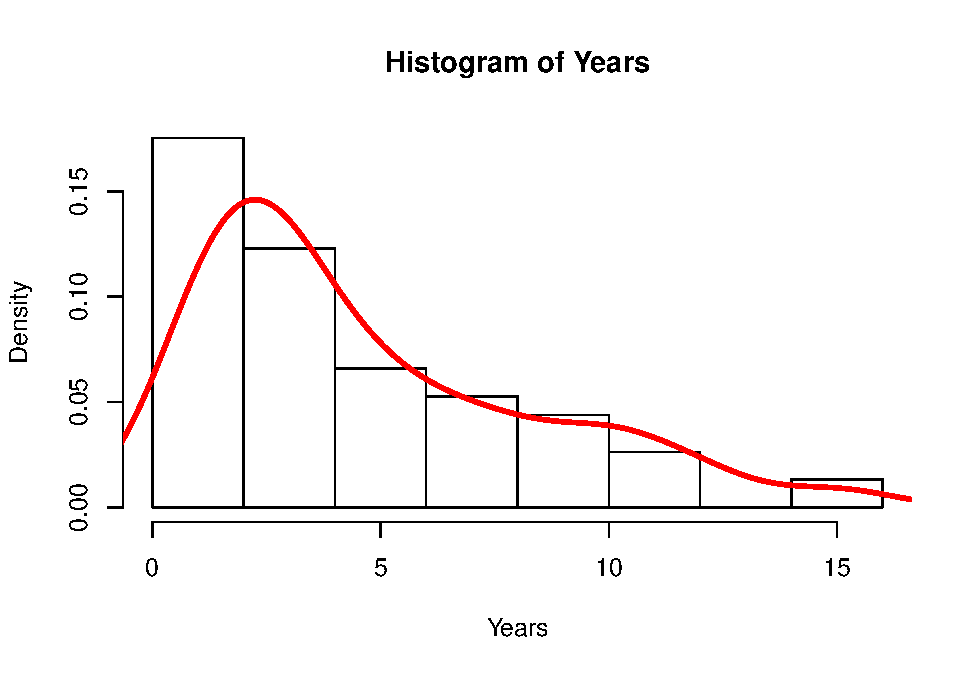
\includegraphics{GreenwoodBanner_files/figure-latex/Figure2-2-1.pdf}
\caption{\label{fig:Figure2-2}Histogram and density curve of Years data.}
\end{figure}

Histograms can be sensitive to the choice of the number of bars and even
the cut-offs used to define the bins for a given number of bars. Small
changes in the definition of cut-offs for the bins can have noticeable
impacts on the shapes observed but this does not impact density curves.
We are not going to tinker with the default choices for bars in
histogram as they are reasonably selected, but we can add information on
the original observations being included in each bar to better
understand the choices that \texttt{hist} is making. In the previous
display, we can add what is called a \textbf{\emph{rug}} to the plot,
were a tick mark is made on the x-axis for each observation. Because the
responses were provided as whole years (1, 2, 3, \ldots{}, 15), we need
to use a graphical technique called \textbf{\emph{jittering}} to add a
little noise\footnote{Jittering typically involves adding random
  variability to each observation that is uniformly distributed in a
  range determined based on the spacing of the function, the results
  will change. For more details, type \texttt{help(jitter)}\\
  in R.} to each observation so all the observations at each year value
do not plot as a single line. In Figure \ref{fig:Figure2-3}, the added
tick marks on the x-axis show the approximate locations of the original
observations. We can see how there are 3 observations at 15 (all were 15
and the noise added makes it possible to see them all). The limitations
of the histogram arise around the 10 year sentence area where there are
many responses at 10 years and just one at both 9 and 11 years, but the
histogram bars sort of miss this that aspect of the data set. The
density curve did show a small bump at 10 years. Density curves are,
however, not perfect and this one shows area for sentences less than 0
years which is not possible here.




\begin{Shaded}
\begin{Highlighting}[]
\KeywordTok{hist}\NormalTok{(MockJury$Years, }\DataTypeTok{freq=}\NormalTok{F, }\DataTypeTok{xlab=}\StringTok{"Years"}\NormalTok{,}
     \DataTypeTok{main=}\StringTok{"Histogram of Years with density curve and rug"}\NormalTok{)}
\KeywordTok{lines}\NormalTok{(}\KeywordTok{density}\NormalTok{(MockJury$Years),}\DataTypeTok{lwd=}\DecValTok{3}\NormalTok{,}\DataTypeTok{col=}\StringTok{"red"}\NormalTok{)}
\KeywordTok{rug}\NormalTok{(}\KeywordTok{jitter}\NormalTok{(MockJury$Years),}\DataTypeTok{col=}\StringTok{"blue"}\NormalTok{,}\DataTypeTok{lwd=}\DecValTok{2}\NormalTok{)}
\end{Highlighting}
\end{Shaded}

\begin{figure}[htbp]
\centering
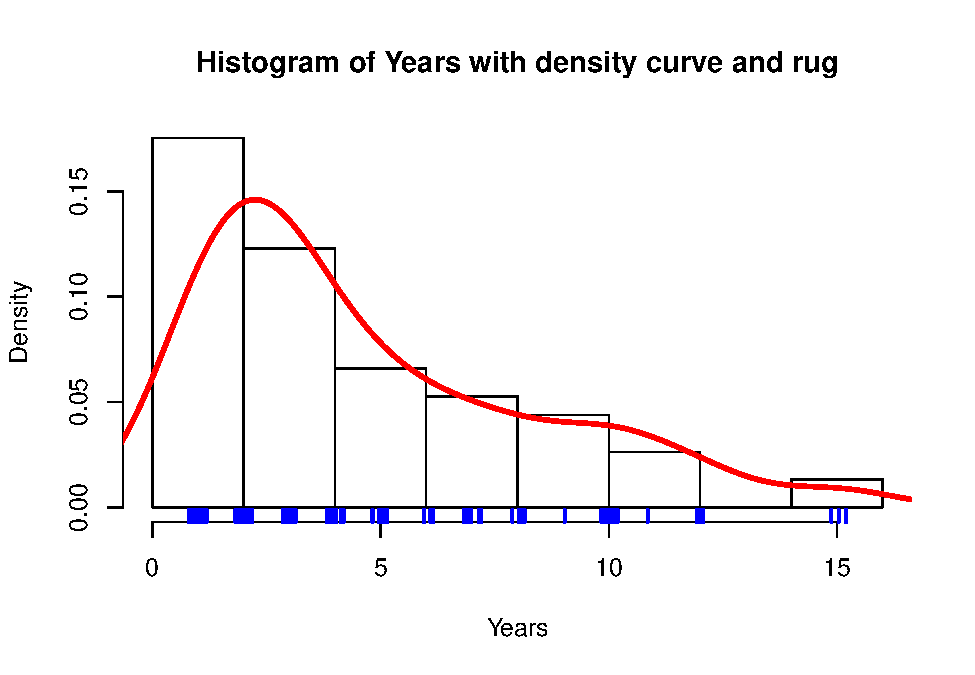
\includegraphics{GreenwoodBanner_files/figure-latex/Figure2-3-1.pdf}
\caption{\label{fig:Figure2-3}Histogram with density curve and rug plot of the jittered
responses.}
\end{figure}

The graphical tools we've just discussed are going to help us move to
comparing the distribution of responses across more than one group. We
will have two displays that will help us make these comparisons. The
simplest is \emph{the \textbf{side-by-side boxplot}}, where a boxplot is
displayed for each group of interest using the same y-axis scaling. In
R, we can use its \textbf{\emph{formula}} notation to see if the
response (\texttt{Years}) differs based on the group (\texttt{Attr}) by
using something like \texttt{Y\textasciitilde{}X} or, here,
\texttt{Years\textasciitilde{}Attr} . We also need to tell R where to
find the variables -- use the last option in the command,
\texttt{data=DATASETNAME} , to inform R of the data.frame to look in to
find the variables. In this example, \texttt{data=MockJury}. We will use
the formula and \texttt{data=...} options in almost every function we
use from here forward. Figure \ref{fig:Figure2-4} contains the
side-by-side boxplots showing right skew for all the groups, slightly
higher median and more variability for the \emph{Unattractive} group
along with some potential outliers indicated in two of the three groups.



\begin{Shaded}
\begin{Highlighting}[]
\KeywordTok{boxplot}\NormalTok{(Years~Attr,}\DataTypeTok{data=}\NormalTok{MockJury)}
\end{Highlighting}
\end{Shaded}

\begin{figure}[htbp]
\centering
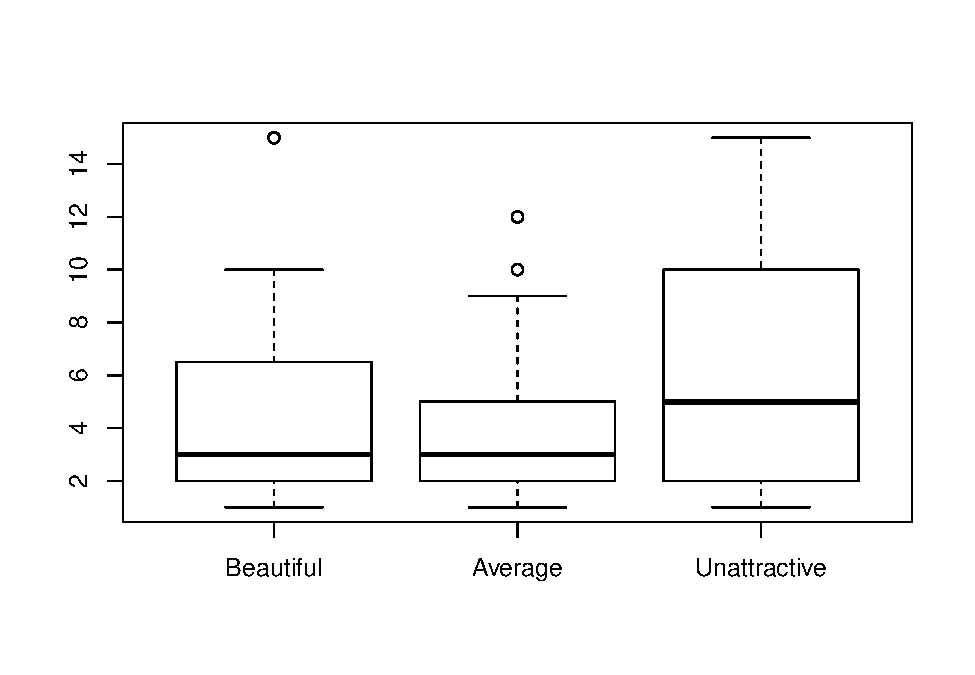
\includegraphics{GreenwoodBanner_files/figure-latex/Figure2-4-1.pdf}
\caption{\label{fig:Figure2-4}Side-by-side boxplot of Years based on picture groups.}
\end{figure}

The ``\textasciitilde{}'' (which is read as the \emph{tilde} symbol,
which you can find in the upper left corner of your keyboard) notation
will be used in two ways this semester. The formula use in R employed
previously declares that the response variable here is \emph{Years} and
the explanatory variable is \emph{Attr}. The other use for
``\textasciitilde{}'' is as shorthand for ``is distributed as'' and is
used in the context of \texttt{Y\textasciitilde{}N(0,1)}, which
translates (in statistics) to defining the random variable \emph{Y} as
following a Normal distribution\footnote{Remember the bell-shaped curve
  you encountered in introductory statistics? If not, you can see some
  at \url{https://en.wikipedia.org/wiki/Normal_distribution}} with mean
0 and standard deviation of 1. In the current situation, we could ask
whether the \texttt{Years} variable seems like it may follow a normal
distribution, in other words, is
\emph{Years}\texttt{\textasciitilde{}N(0,1)}? Since the responses are
right skewed with some groups having outliers, it is not reasonable to
assume that the \emph{Years} variable for any of the three groups may
follow a Normal distribution (more later on the issues this creates!).
Remember that\\
\(\mu\) and \(\sigma\) are parameters where\\
\(\mu\) (``mu'') is our standard symbol for the \textbf{\emph{population
mean}} and that \(\sigma\) (``sigma'') is the symbol of the\\
\textbf{\emph{population standard deviation}}.

\section{Beanplots}\label{section_2-2}

The other graphical display for comparing multiple groups we will use is
a newer display called a \textbf{\emph{beanplot}} (Kampstra, 2008).
Figure \ref{fig:Figure2-5} shows an example of a beanplot that provides
a side-by-side display that contains the density curves, the original
observations that generated the density curve in a (jittered) rug-plot,
the mean of each group, and the overall mean of the entire data set. For
each group, the density curves are mirrored to aid in visual assessment
of the shape of the distribution, which makes a ``bean'' in some cases.
This mirroring also creates a shape that resembles a violin with skewed
distributions so this display has also been called a ``violin plot''.
The innovation in the beanplot is to add bold horizontal lines at the
mean for each group. It also adds a lighter dashed line for the overall
mean. All together this plot shows us information on the center (mean),
spread, and shape of the distributions of the responses. Our inferences
typically focus on the means of the groups and this plot allows us to
compare those across the groups while gaining information on the shapes
of the distributions of responses in each group.

To use the \texttt{beanplot} function we need to install and load the
\texttt{beanplot} package. The function works like the boxplot used
previously except that options for \texttt{log}, \texttt{col}, and
\texttt{method} need to be specified. Use these\footnote{Well, you can
  use other colors (try ``lightblue'' for example), but I think bisque
  looks nice in these plots.} options for any beanplots you make:
\texttt{log="",\ col="bisque",\ method="jitter"}




\begin{Shaded}
\begin{Highlighting}[]
\KeywordTok{require}\NormalTok{(beanplot)}
\KeywordTok{beanplot}\NormalTok{(Years~Attr,}\DataTypeTok{data=}\NormalTok{MockJury,}\DataTypeTok{log=}\StringTok{""}\NormalTok{,}\DataTypeTok{col=}\StringTok{"bisque"}\NormalTok{,}\DataTypeTok{method=}\StringTok{"jitter"}\NormalTok{)}
\end{Highlighting}
\end{Shaded}

\begin{figure}[htbp]
\centering
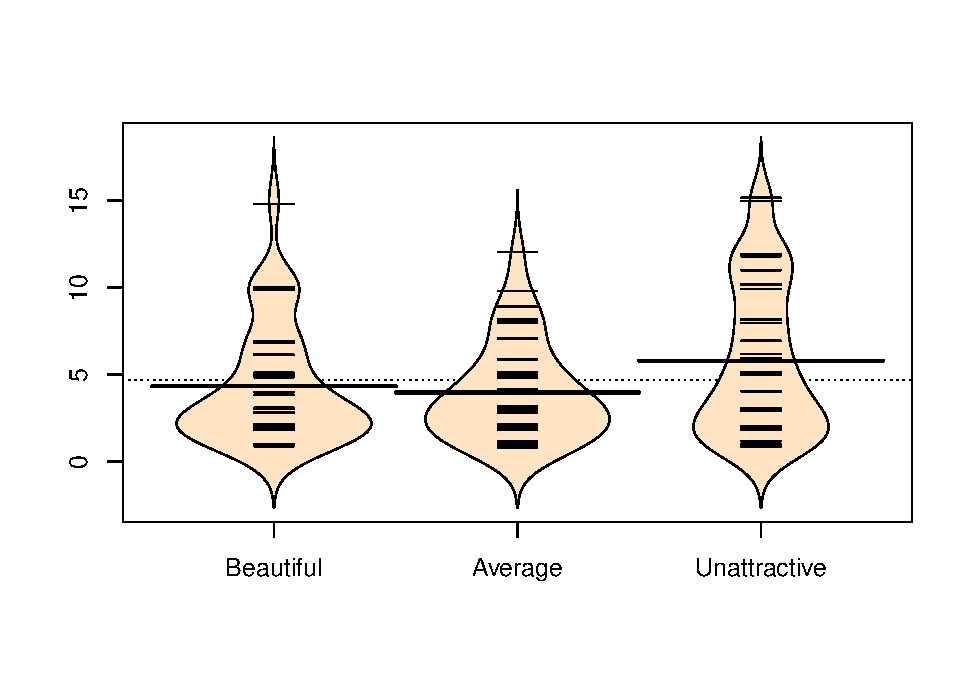
\includegraphics{GreenwoodBanner_files/figure-latex/Figure2-5-1.pdf}
\caption{\label{fig:Figure2-5}Beanplot of Years by picture group. Long, bold lines
correspond to mean of each group.}
\end{figure}

Figure \ref{fig:Figure2-5} reinforces the strong right skews that were
also detected in the boxplots previously. The three large sentences of
15 years can now be clearly identified, with one in the \emph{Beautiful}
group and two in the \emph{Unattractive} group. The \emph{Unattractive}
group seems to have more high observations than the other groups even
though the \emph{Beautiful} group had the largest number of observations
around 10years. The mean sentence was highest for the
\emph{Unattractive} group and the difference in the means between
\emph{Beautiful} and \emph{Average} was small.

In this example, it appears that the mean for \emph{Unattractive} is
larger than the other two groups. But is this difference real? We will
never know the answer to that question, but we can assess how likely we
are to have seen a result as extreme or more extreme than our result,
assuming that there is no difference in the means of the groups. And if
the observed result is (extremely) unlikely to occur, then we can reject
the hypothesis that the groups have the same mean and conclude that
there is evidence of a real difference. To start exploring whether there
are differences in the means, we need to have numerical values to
compare. We can get means and standard deviations by groups easily using
the same formula notation with the \texttt{mean} and \texttt{sd}
functions if the \texttt{mosaic} package is loaded.

\begin{Shaded}
\begin{Highlighting}[]
\KeywordTok{mean}\NormalTok{(Years ~}\StringTok{ }\NormalTok{Attr, }\DataTypeTok{data =} \NormalTok{MockJury)}
\end{Highlighting}
\end{Shaded}

\begin{verbatim}
##    Beautiful      Average Unattractive 
##     4.333333     3.973684     5.810811
\end{verbatim}

\begin{Shaded}
\begin{Highlighting}[]
\KeywordTok{sd}\NormalTok{(Years ~}\StringTok{ }\NormalTok{Attr, }\DataTypeTok{data =} \NormalTok{MockJury)}
\end{Highlighting}
\end{Shaded}

\begin{verbatim}
##    Beautiful      Average Unattractive 
##     3.405362     2.823519     4.364235
\end{verbatim}

We can also use the \texttt{favstats} function to get those summaries
and others.

\begin{Shaded}
\begin{Highlighting}[]
\KeywordTok{favstats}\NormalTok{(Years ~}\StringTok{ }\NormalTok{Attr, }\DataTypeTok{data =} \NormalTok{MockJury)}
\end{Highlighting}
\end{Shaded}

\begin{verbatim}
##           Attr min Q1 median   Q3 max     mean       sd  n missing
## 1    Beautiful   1  2      3  6.5  15 4.333333 3.405362 39       0
## 2      Average   1  2      3  5.0  12 3.973684 2.823519 38       0
## 3 Unattractive   1  2      5 10.0  15 5.810811 4.364235 37       0
\end{verbatim}

Based on these results, we can see that there is an estimated difference
of almost 2 years in the mean sentence between \emph{Average} and
\emph{Unattractive} groups. Because there are three groups being
compared in this study, we will have to wait until Chapter 3 and the
One-Way ANOVA test to fully assess evidence related to some difference
among the three groups. For now, we are going to focus on comparing the
mean \emph{Years} between \emph{Average} and \emph{Unattractive} groups
-- which is a \textbf{\emph{2 independent sample mean}} situation and
something you should have seen before. Remember that the ``independent''
sample part of this refers to observations that are independently
observed for the two groups as opposed to the paired sample situation
that you may have explored where one observation from the first group is
related to an observation in the second group (repeated measures on the
same person or the famous ``twin'' studies with one twin assigned to
each group).

Here we are going to use the ``simple'' two independent group scenario
to review some basic statistical concepts and connect two different
frameworks for conducting statistical inference: randomization and
parametric inference techniques. \textbf{\emph{Parametric}} statistical
methods involve making assumptions about the distribution of the
responses and obtaining confidence intervals and/or p-values using a
\emph{named} distribution (like the z or \emph{t}-distributions).
Typically these results are generated using formulas and looking up
areas under curves or cutoffs using a table or a computer.
\textbf{\emph{Randomization}}-based statistical methods use a computer
to shuffle, sample, or simulate observations in ways that allow you to
obtain distributions of possible results to find areas and cutoffs
without resorting to using tables and named distributions. Randomization
methods are what are called \textbf{\emph{nonparametric}} methods that
often make fewer assumptions (they are \textbf{\emph{not free of
assumptions}}!) and so can handle a larger set of problems more easily
than parametric methods. When the assumptions involved in the parametric
procedures are met by a data set, the randomization methods often
provide very similar results to those provided by the parametric
techniques. To be a more sophisticated statistical consumer, it is
useful to have some knowledge of both of these approaches to statistical
inference and the fact that they can provide similar results might
deepen your understanding of both approaches.

We will start with comparing the \emph{Average} and \emph{Unattractive}
groups to compare these two ways of doing inference. We could remove the
\emph{Beautiful} group observations in a spreadsheet program and read
that new data set back into R, but it is actually pretty easy to use R
to do data management once the data set is loaded. To remove the
observations that came from the \emph{Beautiful} group, we are going to
generate a new variable that we will call \texttt{NotBeautiful} that is
true when observations came from another group (\emph{Average} or
\emph{Unattractive}) and false for observations from the
\emph{Beautiful} group. To do this, we will apply the \textbf{\emph{not
equal}} logical function (\texttt{!=} ) to the variable \texttt{Attr},
inquiring whether it was different from the \texttt{"Beautiful"} level.
You can see the content of the new variable in the output:

\begin{Shaded}
\begin{Highlighting}[]
\NormalTok{MockJury$NotBeautiful <-}\StringTok{ }\NormalTok{MockJury$Attr !=}\StringTok{ "Beautiful"}
\NormalTok{MockJury$NotBeautiful}
\end{Highlighting}
\end{Shaded}

\begin{verbatim}
##   [1] FALSE FALSE FALSE FALSE FALSE FALSE FALSE FALSE FALSE FALSE FALSE
##  [12] FALSE FALSE FALSE FALSE FALSE FALSE FALSE FALSE FALSE FALSE  TRUE
##  [23]  TRUE  TRUE  TRUE  TRUE  TRUE  TRUE  TRUE  TRUE  TRUE  TRUE  TRUE
##  [34]  TRUE  TRUE  TRUE  TRUE  TRUE  TRUE  TRUE  TRUE  TRUE  TRUE  TRUE
##  [45]  TRUE  TRUE  TRUE  TRUE  TRUE  TRUE  TRUE  TRUE  TRUE  TRUE  TRUE
##  [56]  TRUE  TRUE  TRUE  TRUE  TRUE  TRUE  TRUE  TRUE  TRUE  TRUE  TRUE
##  [67]  TRUE  TRUE  TRUE  TRUE  TRUE  TRUE  TRUE  TRUE  TRUE  TRUE FALSE
##  [78] FALSE FALSE FALSE FALSE FALSE FALSE FALSE FALSE FALSE FALSE FALSE
##  [89] FALSE FALSE FALSE FALSE FALSE FALSE  TRUE  TRUE  TRUE  TRUE  TRUE
## [100]  TRUE  TRUE  TRUE  TRUE  TRUE  TRUE  TRUE  TRUE  TRUE  TRUE  TRUE
## [111]  TRUE  TRUE  TRUE  TRUE
\end{verbatim}

This new variable is only FALSE for the \emph{Beautiful} responses as we
can see if we compare some of the results from the original and new
variable:

\begin{Shaded}
\begin{Highlighting}[]
\KeywordTok{head}\NormalTok{(}\KeywordTok{data.frame}\NormalTok{(MockJury$Attr, MockJury$NotBeautiful))}
\end{Highlighting}
\end{Shaded}

\begin{verbatim}
##   MockJury.Attr MockJury.NotBeautiful
## 1     Beautiful                 FALSE
## 2     Beautiful                 FALSE
## 3     Beautiful                 FALSE
## 4     Beautiful                 FALSE
## 5     Beautiful                 FALSE
## 6     Beautiful                 FALSE
\end{verbatim}

\begin{Shaded}
\begin{Highlighting}[]
\KeywordTok{tail}\NormalTok{(}\KeywordTok{data.frame}\NormalTok{(MockJury$Attr, MockJury$NotBeautiful))}
\end{Highlighting}
\end{Shaded}

\begin{verbatim}
##     MockJury.Attr MockJury.NotBeautiful
## 109       Average                  TRUE
## 110       Average                  TRUE
## 111       Average                  TRUE
## 112       Average                  TRUE
## 113       Average                  TRUE
## 114       Average                  TRUE
\end{verbatim}

To get rid of one of the groups, we need to learn a little bit about
data management in R. \textbf{\emph{Brackets}} \texttt{({[},\ {]})} are
used to modify the rows or columns in a data.frame with entries before
the comma operating on rows and entries after the comma on the columns.
For example, if you want to see the results for the 5\(^{th}\) subject,
you can reference the 5\(^{th}\) row of the data.frame using
\texttt{{[}5,\ {]}} after the data.frame name:

\begin{Shaded}
\begin{Highlighting}[]
\NormalTok{MockJury[}\DecValTok{5}\NormalTok{,]}
\end{Highlighting}
\end{Shaded}

\begin{verbatim}
##        Attr    Crime Years Serious exciting calm independent sincere warm
## 5 Beautiful Burglary     7       9        1    1           5       1    8
##   phyattr sociable kind intelligent strong sophisticated happy ownPA
## 5       8        9    4           7      9             9     8     7
##   NotBeautiful
## 5        FALSE
\end{verbatim}

We could just extract the \emph{Years} response for the 5\(^{th}\)
subject by incorporating information on the row and column of interest
(\texttt{Years} is the 3\(^{rd}\) column):

\begin{Shaded}
\begin{Highlighting}[]
\NormalTok{MockJury[}\DecValTok{5}\NormalTok{,}\DecValTok{3}\NormalTok{]}
\end{Highlighting}
\end{Shaded}

\begin{verbatim}
## [1] 7
\end{verbatim}

In R, we can use logical vectors to keep any rows of the data.frame
where the variable is true and drop any rows where it is false by
placing the logical variable in the first element of the brackets. The
reduced version of the data set should be saved with a different name
such as \texttt{MockJury2} that is used here to reduce the chances of
confusing it with the previous full data set:

\begin{Shaded}
\begin{Highlighting}[]
\NormalTok{MockJury2 <-}\StringTok{ }\NormalTok{MockJury[MockJury$NotBeautiful,]}
\end{Highlighting}
\end{Shaded}

You will always want to check that the correct observations were dropped
either using \texttt{View(MockJury2)} or by doing a quick summary of the
\texttt{Attr} variable in the new data.frame.

\begin{Shaded}
\begin{Highlighting}[]
\KeywordTok{summary}\NormalTok{(MockJury2$Attr)}
\end{Highlighting}
\end{Shaded}

\begin{verbatim}
##    Beautiful      Average Unattractive 
##            0           38           37
\end{verbatim}

It ends up that R remembers the \emph{Beautiful} category even though
there are 0 observations in it now and that can cause us some problems.
When we remove a group of observations, we sometimes need to clean up
categorical variables to just reflect the categories that are present.
The \texttt{factor} function creates categorical variables based on the
levels of the variables that are observed and is useful to run here to
clean up \texttt{Attr}.

\begin{Shaded}
\begin{Highlighting}[]
\NormalTok{MockJury2$Attr <-}\StringTok{ }\KeywordTok{factor}\NormalTok{(MockJury2$Attr) }
\KeywordTok{summary}\NormalTok{(MockJury2$Attr)}
\end{Highlighting}
\end{Shaded}

\begin{verbatim}
##      Average Unattractive 
##           38           37
\end{verbatim}

Now if we remake the boxplots and beanplots, they only contain results
for the two groups of interest here as seen in Figure
\ref{fig:Figure2-6}.




\begin{Shaded}
\begin{Highlighting}[]
\KeywordTok{boxplot}\NormalTok{(Years ~}\StringTok{ }\NormalTok{Attr,}\DataTypeTok{data=}\NormalTok{MockJury2) }
\KeywordTok{beanplot}\NormalTok{(Years ~}\StringTok{ }\NormalTok{Attr,}\DataTypeTok{data=}\NormalTok{MockJury2,}\DataTypeTok{log=}\StringTok{""}\NormalTok{,}\DataTypeTok{col=}\StringTok{"bisque"}\NormalTok{,}\DataTypeTok{method=}\StringTok{"jitter"}\NormalTok{)}
\end{Highlighting}
\end{Shaded}

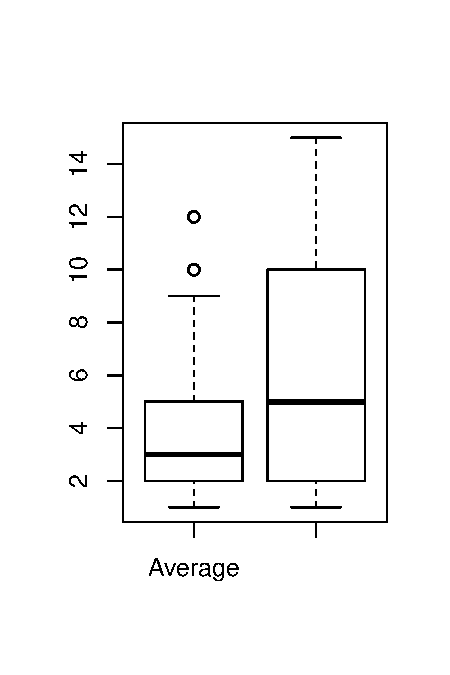
\includegraphics{GreenwoodBanner_files/figure-latex/Figure2-6-1.pdf}
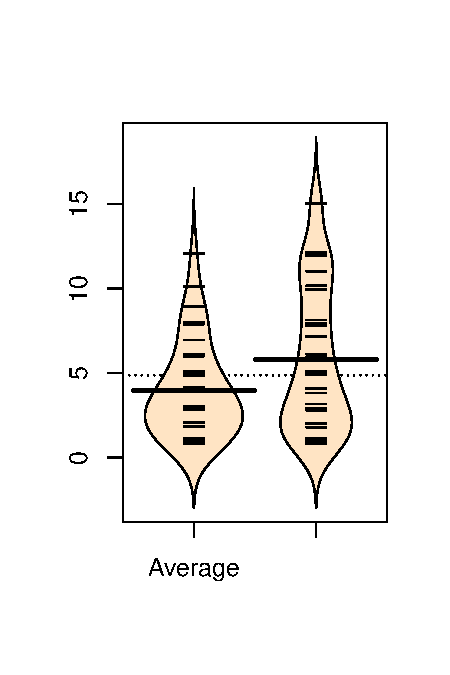
\includegraphics{GreenwoodBanner_files/figure-latex/Figure2-6-2.pdf}

The two-sample mean techniques you learned in your previous course all
start with comparing the means the two groups. We can obtain the two
means using the \texttt{mean} function or directly obtain the difference
in the means using the \texttt{diffmean} function (both require the
\texttt{mosaic} package). The \texttt{diffmean} function provides
\(\bar{x}_{Unattractive} - \bar{x}_{Average}\) where \(\bar{x}\) (read
as ``x-bar'') is the sample mean ofobservations in the subscripted
group. Note that there are two directions that you could compare the
means and this function chooses to take the mean from the second group
name \emph{alphabetically} and subtract the mean from the first
alphabetical group name. It is always good to check the direction of
this calculation as having a difference of \(-1.84\) years versus
\(1.84\) years could be important.

\begin{Shaded}
\begin{Highlighting}[]
\KeywordTok{mean}\NormalTok{(Years ~}\StringTok{ }\NormalTok{Attr, }\DataTypeTok{data=}\NormalTok{MockJury2)}
\end{Highlighting}
\end{Shaded}

\begin{verbatim}
##      Average Unattractive 
##     3.973684     5.810811
\end{verbatim}

\begin{Shaded}
\begin{Highlighting}[]
\KeywordTok{diffmean}\NormalTok{(Years ~}\StringTok{ }\NormalTok{Attr, }\DataTypeTok{data=}\NormalTok{MockJury2)}
\end{Highlighting}
\end{Shaded}

\begin{verbatim}
## diffmean 
## 1.837127
\end{verbatim}

\section{Models, hypotheses, and permutations for the 2 sample mean
situation}\label{section_2-3}

There appears to be some evidence that the \emph{Unattractive} group is
getting higher average lengths of sentences from the prisoner ``jurors''
than the \emph{Average} group, but we want to make sure that the
difference is real -- that there is evidence to reject the assumption
that the means are the same ``in the population''. First, a
\textbf{\emph{null hypothesis}}\footnote{The hypothesis of no difference
  that is typically generated in the hopes of being rejected in favor of
  the alternative hypothesis which contains the sort of difference that
  is of interest in the application.} which defines a \textbf{\emph{null
model}}\footnote{The null model is the statistical model that is implied
  by the chosen null hypothesis. Here, a null hypothesis of no
  difference translates to having a model with the same mean for both
  groups.} needs to be determined in terms of \textbf{\emph{parameters}}
(the true values in the population). The research question should help
you determine the form of the hypotheses for the assumed population. In
the 2 independent sample mean problem, the interest is in testing a null
hypothesis of \(H_0: \mu_1 = \mu_2\) versus the alternative hypothesis
of \(H_A: \mu_1 \ne \mu_2\), where \(\mu_1\) is the parameter for the
true mean of the first group and \(\mu_2\) is the parameter for the true
mean of the second group. The alternative hypothesis involves assuming a
statistical model for the \(i^{th} (i=1,\ldots,n_j)\) response from the
\(j^{th} (j=1,2)\) group, \(\boldsymbol{y}_{ij}\), that involves
modeling it as \(y_{ij} = \mu_j + \epsilon_{ij}\), where we assume that
\(\epsilon_{ij} \sim N(0,\sigma^2)\). For the moment, focus on the
models that either assume the means are the same (null) or different
(alternative), which imply:

\begin{itemize}
\item
  Null Model: \(y_{ij} = \mu + \epsilon_{ij}\) There is \textbf{no}
  difference in \textbf{true} means for the two groups.
\item
  Alternative Model: \(y_{ij} = \mu_j + \epsilon_{ij}\) There is
  \textbf{a} difference in \textbf{true} means for the two groups.
\end{itemize}

Suppose we are considering thealternative model for the 4th observation
(\(i=4\)) from the second group (\(j=2\)), then the model for this
observation is \(y_{42} = \mu_2 +\epsilon_{42}\), that defines the
response as coming from the true mean for the second group plus a random
error term for that observation, \(\epsilon_{42}\). For, say, the 5th
observation from the first group (\(j=1\)), the model is
\(y_{51} = \mu_1 +\epsilon_{51}\). If we were working with the null
model, the mean is always the same (\(\mu\)) - the group specified does
not change the mean we use for that observation.

It can be helpful to think about the null and alternative models
graphically. By assuming the null hypothesis is true (means are equal)
and that the random errors around the mean follow a normal distribution,
we assume that the truth is as displayed in the left panel of Figure
\ref{fig:Figure2-7} -- two normal distributions with the same mean and
variability. The alternative model allows the two groups to potentially
have different means, such as those displayed in the right panel of
Figure \ref{fig:Figure2-7} where the second group has a larger mean.
Note that in this scenario, we assume that the observations all came
from the same distribution except that they had different means.
Depending on the statistical procedure we are using, we basically are
going to assume that the observations (\(y_{ij}\)) either were generated
as samples from the null or alternative model. You can imagine drawing
observations at random from the pictured distributions. For hypothesis
testing, the null model is assumed to be true and then the unusualness
of the actual result is assessed relative to that assumption. In
hypothesis testing, we have to decide if we have enough evidence to
reject the assumption that the null model (or hypothesis) is true. If we
reject the null hypothesis, then we would conclude that the other model
considered (the alternative model) is more reasonable. The researchers
obviously would have hoped to encounter some sort of noticeable
difference in the sentences provided for the different pictures and been
able to find enough evidence to reject the null model where the groups
``look the same''.





\begin{figure}
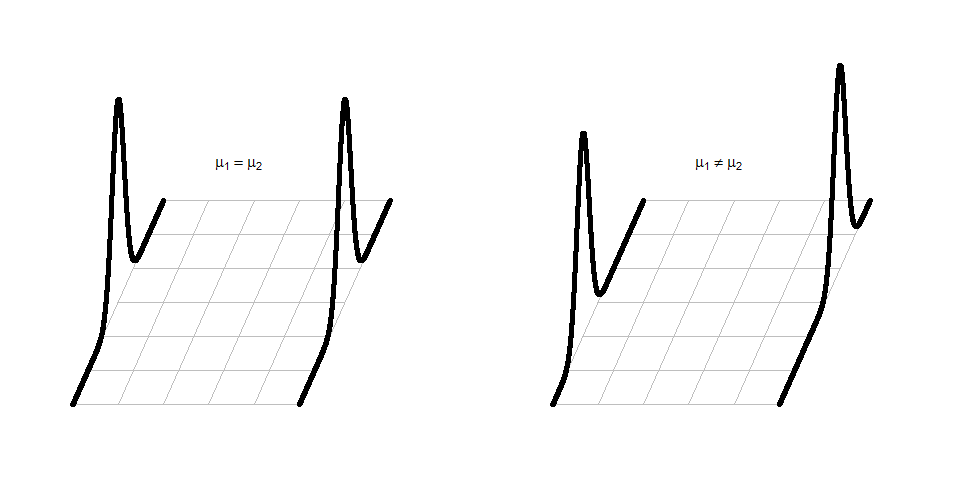
\includegraphics[width=13.33in]{chapter1_files/image015} \caption{Illustration of the assumed situations under the null
(left) and a single possibility that could occur if the alternative were
true (right) and the true means were different.}\label{fig:Figure2-7}
\end{figure}

In statistical inference, null hypotheses (and their implied models) are
set up as ``straw men'' with every interest in rejecting them even
though we assume they are true to be able to assess the evidence against
them. Consider the original study design here, the pictures were
randomly assigned to the subjects. If the null hypothesis were true,
then we would have no difference in the population means of the groups.
And this would apply if we had done a different random assignment of the
pictures to the subjects. So let's try this: assume that the null
hypothesis is true and randomly re-assign the treatments (pictures) to
the observations that were obtained. In other words, keep the sentences
(\emph{Years}) the same and shuffle the group labels randomly. The
technical term for this is doing a \textbf{\emph{permutation}} (a random
shuffling of the treatments relative to the responses). If the null is
true and the means in the two groups are the same, then we should be
able to re-shuffle the groups to the observed sentences (\emph{Years})
and get results similar to those we actually observed. If the null is
false and the means are really different in the two groups, then what we
observed should differ from what we get under other random permutations.
The differences between the two groups should be more noticeable in the
observed data set than in (most) of the shuffled data sets. It helps to
see an example of a permutation of the labels to understand what this
means here.

In the \texttt{mosaic} package, the \texttt{shuffle} function allows us
to easily perform a permutation\footnote{We'll see the \texttt{shuffle}
  function in a more common usage below; while the code to generate
  \texttt{Perm1} is provided, it isn't something to worry about right
  now.}. Just one time, we can explore what a permutation of the
treatment labels could look like in the \texttt{PermutedAttr} variable
below. Note that the \texttt{Years} are held in the same place the group
labels are shuffled.

\begin{Shaded}
\begin{Highlighting}[]
\NormalTok{Perm1 <-}\StringTok{ }\KeywordTok{with}\NormalTok{(MockJury2,}\KeywordTok{data.frame}\NormalTok{(Years,Attr,}\DataTypeTok{PermutedAttr=}\KeywordTok{shuffle}\NormalTok{(Attr)))}
\NormalTok{Perm1}
\end{Highlighting}
\end{Shaded}

\begin{verbatim}
##    Years         Attr PermutedAttr
## 1      1 Unattractive      Average
## 2      4 Unattractive      Average
## 3      3 Unattractive      Average
## 4      2 Unattractive Unattractive
## 5      8 Unattractive Unattractive
## 6      8 Unattractive      Average
## 7      1 Unattractive      Average
## 8      1 Unattractive Unattractive
## 9      5 Unattractive Unattractive
## 10     7 Unattractive Unattractive
## 11     1 Unattractive      Average
## 12     5 Unattractive      Average
## 13     2 Unattractive Unattractive
## 14    12 Unattractive      Average
## 15    10 Unattractive Unattractive
## 16     1 Unattractive      Average
## 17     6 Unattractive Unattractive
## 18     2 Unattractive Unattractive
## 19     5 Unattractive      Average
## 20    12 Unattractive      Average
## 21     6 Unattractive      Average
## 22     3 Unattractive Unattractive
## 23     8 Unattractive      Average
## 24     4 Unattractive Unattractive
## 25    10 Unattractive      Average
## 26    10 Unattractive      Average
## 27    15 Unattractive      Average
## 28    15 Unattractive      Average
## 29     3 Unattractive      Average
## 30     3 Unattractive Unattractive
## 31     3 Unattractive      Average
## 32    11 Unattractive      Average
## 33    12 Unattractive Unattractive
## 34     2 Unattractive Unattractive
## 35     1 Unattractive Unattractive
## 36     1 Unattractive      Average
## 37    12 Unattractive      Average
## 38     5      Average Unattractive
## 39     5      Average Unattractive
## 40     4      Average Unattractive
## 41     3      Average Unattractive
## 42     6      Average Unattractive
## 43     4      Average      Average
## 44     9      Average Unattractive
## 45     8      Average      Average
## 46     3      Average      Average
## 47     2      Average      Average
## 48    10      Average Unattractive
## 49     1      Average Unattractive
## 50     1      Average      Average
## 51     3      Average Unattractive
## 52     1      Average Unattractive
## 53     3      Average Unattractive
## 54     5      Average      Average
## 55     8      Average Unattractive
## 56     3      Average Unattractive
## 57     1      Average Unattractive
## 58     1      Average      Average
## 59     1      Average Unattractive
## 60     2      Average Unattractive
## 61     2      Average Unattractive
## 62     1      Average      Average
## 63     1      Average      Average
## 64     2      Average      Average
## 65     3      Average      Average
## 66     4      Average Unattractive
## 67     5      Average Unattractive
## 68     3      Average      Average
## 69     3      Average      Average
## 70     3      Average      Average
## 71     2      Average      Average
## 72     7      Average Unattractive
## 73     6      Average Unattractive
## 74    12      Average Unattractive
## 75     8      Average      Average
\end{verbatim}

If you count up the number of subjects in each group by counting the
number of times each label (Average, Unattractive) occurs, it is the
same in both the \texttt{Attr} and \texttt{PermutedAttr} columns.
Permutations involve randomly re-ordering the values of a variable --
here the \texttt{Attr} group labels -- without changing the content of
the variable. This result can also be generated using what is called
\textbf{\emph{sampling without replacement}}: sequentially select \(n\)
labels from the original variable, removing each used label and making
sure that each original \texttt{Attr} label is selected once and only
once. The new, randomly selected order of selected labels provides the
permuted labels. Stepping through the process helps to understand how it
works: after the initial random sample of one label, there would
\(n - 1\) choices possible; on the \(n^{th}\) selection, there would
only be one label remaining to select. This makes sure that all original
labels are re-used but that the order is random. Sampling without
replacement is like picking names out of a hat, one-at-a-time, and not
putting the names back in after they are selected. It is an exhaustive
process for all the original observations. \textbf{\emph{Sampling with
replacement}} , in contrast, involves sampling from the specified list
with each observation having an equal chance of selection for each
sampled observation -- in other words, observations can be selected more
than once. This is like picking \(n\) names out of a hat that contains
\(n\) names, except that every time a name is selected, it goes back
into the hat -- we'll use this technique in Section @ref(section\_2-8)
to do what is called \textbf{\emph{bootstrapping}} . Both sampling
mechanisms can be used to generate inferences but each has particular
situations where they are most useful. For hypothesis testing, we will
use permutations (sampling without replacement).

The comparison of the beanplots for the real data set and permuted
version of the labels is what is really interesting (Figure
\ref{fig:Figure2-8}). The original difference in the sample means of the
two groups was 1.84 years (Unattractive minus Average). The sample means
are the \textbf{\emph{statistics}}\\
that estimate the parameters for the true means of the two groups. In
the permuted data set, the difference in the means is 1.15 years in the
opposite direction (Average had a higher mean than Unattractive in the
permuted data).

\begin{Shaded}
\begin{Highlighting}[]
\KeywordTok{mean}\NormalTok{(Years ~}\StringTok{ }\NormalTok{PermutedAttr, }\DataTypeTok{data=}\NormalTok{Perm1)}
\end{Highlighting}
\end{Shaded}

\begin{verbatim}
##      Average Unattractive 
##     5.184211     4.567568
\end{verbatim}

\begin{Shaded}
\begin{Highlighting}[]
\KeywordTok{diffmean}\NormalTok{(Years ~}\StringTok{ }\NormalTok{PermutedAttr, }\DataTypeTok{data=}\NormalTok{Perm1)}
\end{Highlighting}
\end{Shaded}

\begin{verbatim}
##  diffmean 
## -0.616643
\end{verbatim}




\begin{verbatim}
## log="y" selected
## log="y" selected
\end{verbatim}

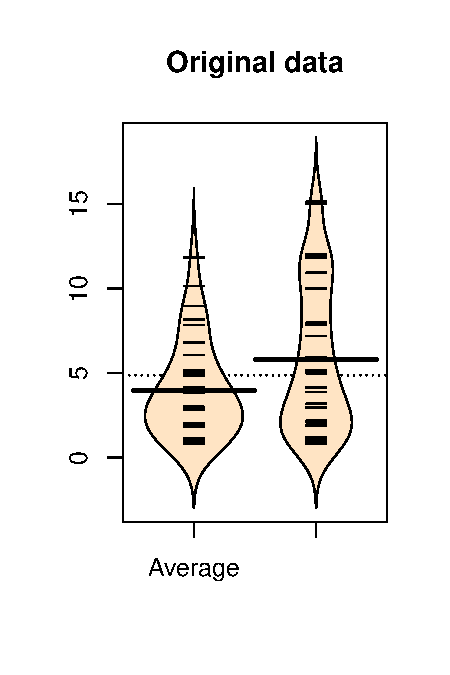
\includegraphics{GreenwoodBanner_files/figure-latex/Figure2-8-1.pdf}
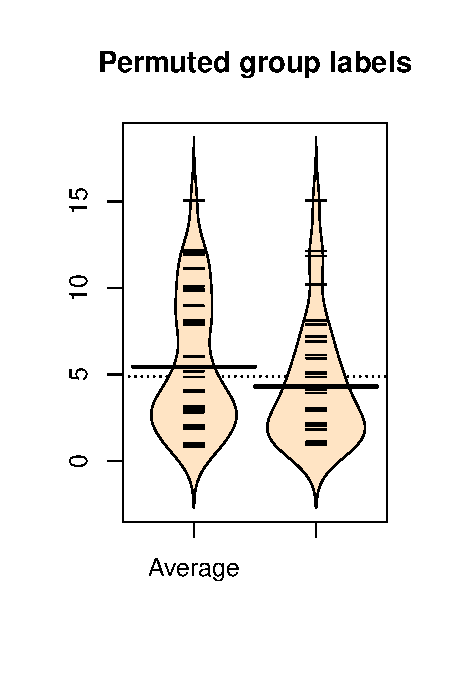
\includegraphics{GreenwoodBanner_files/figure-latex/Figure2-8-2.pdf}

These results suggest that the observed difference was larger than what
we got when we did a single permutation although it was only a little
bit larger than a difference we could observe in permutations if we
ignore the difference in directions. Conceptually, permuting
observations between group labels is consistent with the null hypothesis
-- this is a technique to generate results that we might have gotten if
the null hypothesis were true since the responses are the same in the
two groups if the null is true. We just need to repeat the permutation
process many times and track how unusual our observed result is relative
to this distribution of potential responses if the null were true. If
the observed differences are unusual relative to the results under
permutations, then there is evidence against the null hypothesis, the
null hypothesis should be rejected ( Reject \(H_0\)), and a conclusion
should be made, in the direction of the alternative hypothesis, that
there is evidence that the true means differ. If the observed
differences are similar to (or at least not unusual relative to) what we
get under random shuffling under the null model, we would have a tough
time concluding that there is any real difference between the groups
based on our observed data set.

\section{Permutation testing for the 2 sample mean
situation}\label{section_2-4}

\section{Hypothesis testing (general)}\label{section_2-5}

\section{Connecting randomization (nonparametric) and parametric
tests}\label{section_2-6}

\section{Second example of permutation tests}\label{section_2-7}

\section{Confidence intervals and bootstrapping}\label{section_2-8}

\section{Bootstrap confidence intervals for difference in
GPAs}\label{section_2-9}

\section{Chapter summary}\label{section_2-10}

\section{Summary of important R code}\label{section_2-11}

\section{Practice problems}\label{section_2-12}

\bibliography{packages,book}


\end{document}
